\chapter{系统设计与实现}
\label{ch:method}

\section{架构与项目边界}

系统分为编辑器、资源、运行时和测试四个部分，如图\ref{fig:architecture}所示。游戏通过资源文件和运行组件执行行为树，不依赖编辑器界面。Live Debug 也只出现在 Godot 编辑器中，不会加入最终游戏画面。

\begin{figure}[htbp]
\centering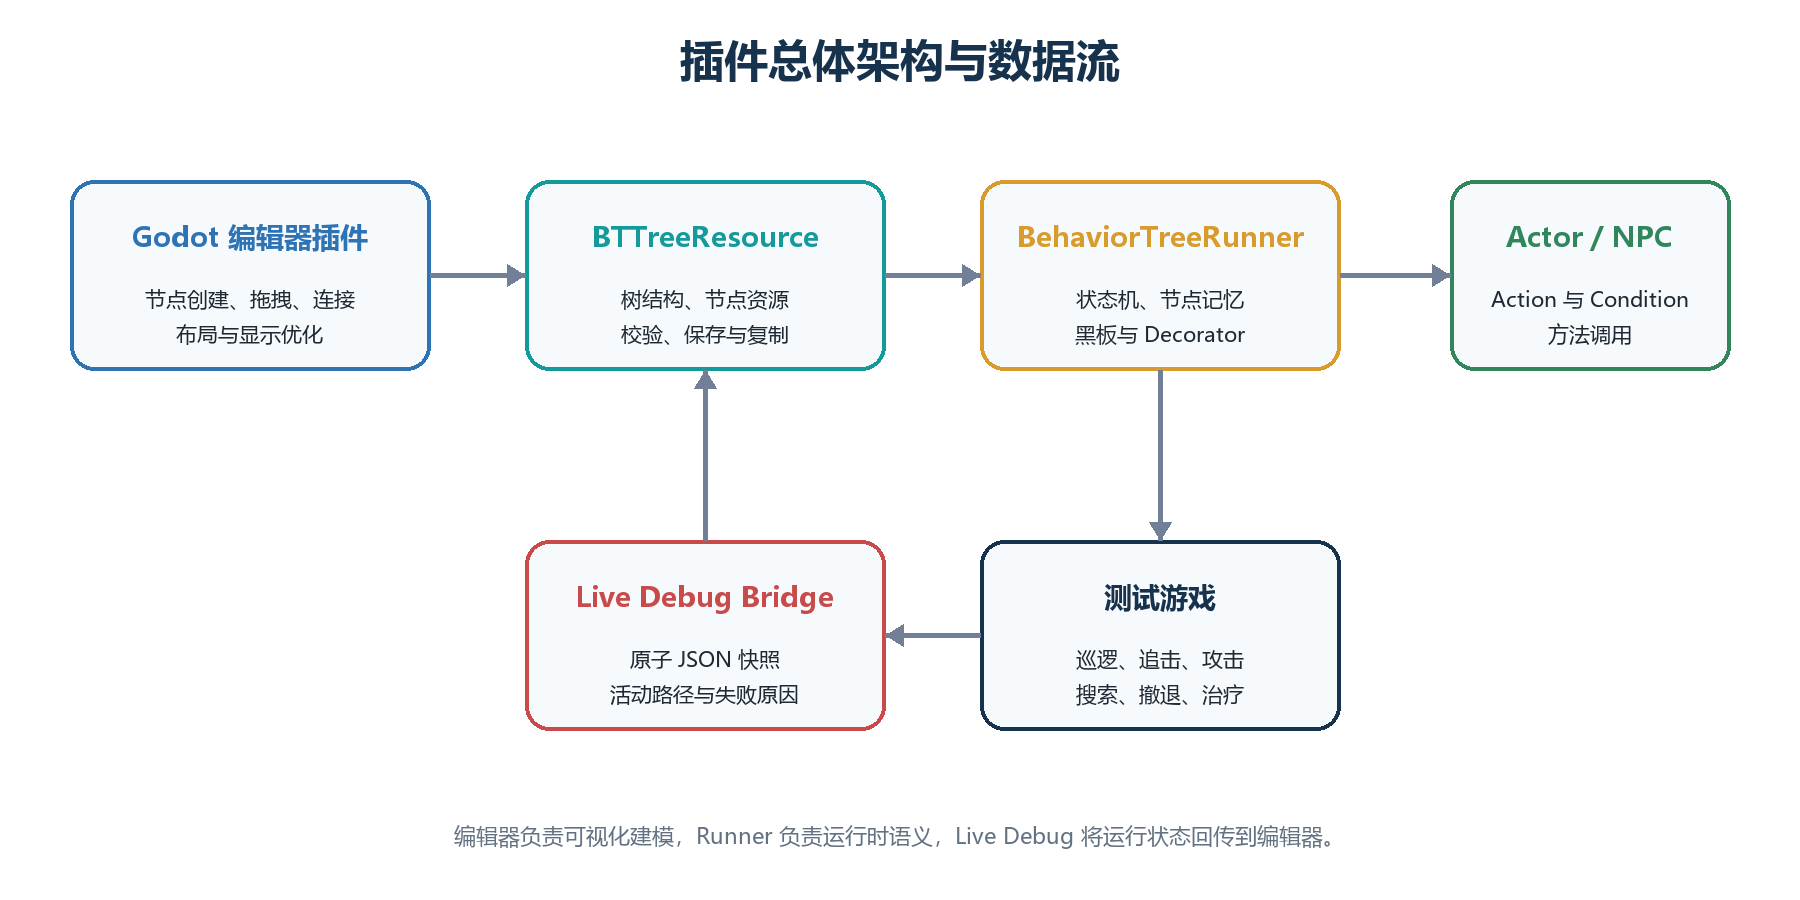
\includegraphics[width=\textwidth]{figures/architecture.png}
\caption{Godot 编辑器、行为树资源、Runner 与 Actor 之间的插件架构和数据流。}
\label{fig:architecture}
\end{figure}

\texttt{BTTreeResource} 保存整棵树，\texttt{BTNodeResource} 保存单个节点的类型、参数、位置和父级关系。\texttt{BehaviorTreeRunner} 负责执行行为树，\texttt{BehaviorTreeComponent} 则把行为树连接到场景中的 Actor。编辑器主界面负责画布、属性编辑、黑板、历史记录和 Live Debug。这样的分工使资源、执行逻辑和显示界面可以分别测试。

\section{资源模型与校验}

普通节点使用 \texttt{parent\_id} 记录父节点，Decorator 使用单独的 \texttt{decorator\_parent\_id}。因此 Decorator 不会被错误地当作普通子节点执行。同级子节点按画布上的横向位置排序，所以从左到右的显示顺序就是执行顺序。保存资源时，节点位置和这个顺序都会被保留。

保存前会检查 Root 是否存在、节点 ID 是否重复、父级是否有效、Decorator 是否正确附着，以及节点参数是否完整。例如，Root 不能有父级，Action 和 Condition 不能拥有普通子节点。编辑器保存和自动测试使用同一套检查规则。

黑板 Schema 可以声明 Bool、Int、Float、String 和 \texttt{Vector2} 类型，并为每个键设置默认值。严格模式会报告未声明或无效的键。Inspector 提供键选择器，同时保留自由输入方式。Schema 修改也进入撤销和重做历史。

\section{运行时语义}

行为树每次更新都会返回 \textsc{success}、\textsc{failure} 或 \textsc{running}。需要跨帧继续执行的节点会按 ID 保存进度；重启、切换行为树或中断分支时会清除这些记录。表\ref{tab:nodes}概括各类节点的行为。

\begin{table}[htbp]
\centering
\caption{已实现的运行时节点语义。}\label{tab:nodes}
\begin{tabular}{p{0.22\textwidth}p{0.68\textwidth}}
\toprule 节点 & 行为 \\
\midrule
Root & 执行唯一普通子节点。\\
Sequence & 按序执行，遇失败或运行停止，并记忆运行索引。\\
Selector & 按序执行，遇成功或运行停止，并记忆运行索引。\\
Reactive Selector & 每 Tick 从高优先级重新检查，可中断低优先级分支。\\
Random Selector & 使用可设种子的随机选择，运行期间保持同一子节点。\\
Parallel & Tick 多个子节点并应用成功/失败阈值。\\
Repeat & 固定次数或无限重复，跨 Tick 保存计数。\\
Wait & 累积 delta，到达时间后成功。\\
Condition & 调用 Actor 判断或比较黑板值。\\
Action & 调用 Actor 方法，把 Bool 或状态转成树状态。\\
\bottomrule
\end{tabular}
\end{table}

Action 和 Actor 模式的 Condition 使用统一接口调用 Actor 方法。如果方法不存在，节点返回失败并显示原因，而不是使游戏崩溃。黑板条件支持键是否存在、真假、相等、不等和数值大小比较。

Decorator 会在所属节点执行前后改变条件或结果。已实现的功能包括黑板比较、冷却时间、时间限制、结果反转、强制结果和重复。重置子树时，Decorator 和子节点保存的运行进度会一起清除。

\section{编辑器编写工作流}

插件显示在 Godot 编辑器底部。用户在画布上点击右键创建节点，不需要在菜单栏中面对一排创建按钮。节点可以移动、连接、断开、复制和删除。行为树选择器只显示资源名称，用户不需要手动查看或输入完整文件路径。创建、删除、移动、连线、参数修改、Schema 修改和折叠状态都支持撤销与重做。

Inspector 使用与字段类型对应的控件。例如，Action 直接填写方法名，Condition 选择 Actor 或黑板模式并设置键、比较方式和值。Random、Parallel、Repeat、Wait 和 Decorator 也有自己的设置项。高级 JSON 只作为兼容入口，不是正常操作的必需步骤。

本插件使用节点上方和下方的连接端口，而 Godot 默认连线主要面向左右端口。因此插件自行绘制正式连线，并在用户拖动连线时使用 Godot 的预览。自定义连线仍可通过右键断开，并支持撤销和重做。关闭自定义显示后可以恢复 Godot 原生连线。

\section{Live Debug 与黑板检查}

运行时会把当前 Actor、行为树、活动节点、执行路径、失败原因和黑板值写入调试文件。文件写完后才会替换旧版本，避免编辑器读到不完整内容。如果一次读取失败，编辑器保留上一份完整状态，并在下一次更新时重试。

编辑器只显示当前行为树的调试信息。活动路径使用明显边框，非活动分支可以淡化，失败节点会显示原因，黑板面板显示当前键和值。较长的路径放在可滚动区域中，避免遮挡主画布。游戏画面中不会出现这些调试内容。

\begin{figure}[htbp]
\centering
\includegraphics[width=0.92\textwidth]{figures/07_runtime_failure.png}
\caption{仅位于编辑器中的活动路径和失败原因显示。}\label{fig:livedebug}
\end{figure}

\section{大型树显示机制}

大型行为树的问题不只来自节点数量，还来自卡片信息、连线密度、导航距离和运行状态同时增加。为此，插件从信息密度、焦点与结构裁剪、导航与概览、连线与运行表示四个方面提供显示功能。

\subsection{信息密度控制}
Compact 缩小卡片，但不隐藏节点。卡片保留节点类型和短标题，参数、描述和 Decorator 摘要可以在需要时再显示。Semantic Zoom 根据画布缩放比例切换信息层级：近距离显示完整字段，中距离保留标题和关键参数，远距离只保留识别节点所需的信息。这两项功能都不会改变行为树资源。

节点类型还使用颜色、图标和形状进行重复编码。即使颜色不容易区分，用户仍可通过图标和轮廓识别 Root、复合节点、任务和 Decorator。插件同时提供色盲友好配色，减少只依赖单一颜色通道的问题。

\begin{figure}[htbp]
\centering
\begin{minipage}{0.48\textwidth}\centering
\includegraphics[width=\linewidth]{figures/01_baseline.png}\\[-1mm]\small (a) 基线\end{minipage}\hfill
\begin{minipage}{0.48\textwidth}\centering
\includegraphics[width=\linewidth]{figures/02_compact.png}\\[-1mm]\small (b) 紧凑卡片\end{minipage}
\caption{同一行为树的完整细节基线和紧凑显示。}\label{fig:compact}
\end{figure}

\subsection{焦点与结构裁剪}
鱼眼 Focus+Context 会放大指针附近的卡片，同时保留周围节点作为位置参考。最大放大倍率限制为 1.20 倍，卡片以自身中心补偿位置，避免放大后整体布局持续漂移。关闭鱼眼后，卡片恢复原来的尺寸和位置。

Search 支持标题、类型、描述、Action、Condition 和 Decorator 参数搜索，并提供上一个、下一个和清除操作。匹配节点保持明显，其他节点淡化，选定目标可以移动到当前视口。Subtree Focus 只显示指定分支和必要上下文；Context Collapse 保留折叠根和隐藏节点摘要，但暂时不绘制后代。展开后仍使用原有节点位置和父子关系。

\begin{figure}[htbp]
\centering
\begin{minipage}{0.48\textwidth}\centering
\includegraphics[width=\linewidth]{figures/03_fisheye.png}\\[-1mm]\small (a) 鱼眼焦点与上下文\end{minipage}\hfill
\begin{minipage}{0.48\textwidth}\centering
\includegraphics[width=\linewidth]{figures/05_collapsed.png}\\[-1mm]\small (b) 子树折叠与摘要\end{minipage}
\caption{局部放大和结构裁剪的两种实现。}\label{fig:focuscollapse}
\end{figure}

\subsection{导航与概览}
增强小地图使用固定区域显示整棵树的缩略结构，并标出当前视口位置。Fit 用于把当前图形移动到可查看范围，Focus 用于定位选中节点，Show All 用于取消局部显示并返回完整树。Breadcrumb 显示从 Root 到当前节点的层级路径，路径摘要则以文字形式给出当前执行或选择路径，因此在卡片缩小时仍可确认所处位置。

搜索结果可以使用按钮或键盘在前后目标之间移动。多列布局把拥有大量子节点的分支分成多列，避免单层无限向横向扩展；稳定布局尽量保留未修改分支的位置，减少一次编辑造成的大范围移动。自动排列仍保持同级节点从左到右的执行顺序。

\begin{figure}[htbp]
\centering
\includegraphics[width=0.92\textwidth]{figures/10_complex_tree.png}
\caption{复杂树中的小地图、路径摘要、导航控件和自动布局。}\label{fig:navigation}
\end{figure}

\subsection{连线与运行表示}
插件使用节点下方的输出端口和上方的输入端口表达父子关系。正式连线由插件自行绘制，拖动预览仍使用 Godot 的 GraphEdit 输入处理。正交连线使用水平和垂直线段减少曲线交叉；边捆绑让具有共同父级的连线先共享一段主干，再分向各个子节点。两种方式都保留连线点击、断开、撤销和重做。

运行时表示在同一画布上显示活动路径、当前节点、成功或失败状态、非活动分支淡化和失败原因。路径颜色沿父子关系连续传播，Decorator 失败会显示在所属节点附近。这样，用户既能看到静态结构，也能看到本次 Tick 实际经过的分支。

\begin{figure}[htbp]
\centering
\begin{minipage}{0.48\textwidth}\centering
\includegraphics[width=\linewidth]{figures/08_orthogonal_edges.png}\\[-1mm]\small (a) 正交连线与活动路径\end{minipage}\hfill
\begin{minipage}{0.48\textwidth}\centering
\includegraphics[width=\linewidth]{figures/09_bundled_edges.png}\\[-1mm]\small (b) 边捆绑与失败标注\end{minipage}
\caption{连线组织和运行状态表示。}\label{fig:edgesruntime}
\end{figure}

\section{物理屏幕实验基础设施}

屏幕测试工具读取 EDID 中的物理宽高，并将它与分辨率分开记录。对于宽 \(W_{\mathrm{cm}}\)、高 \(H_{\mathrm{cm}}\) 的屏幕，测试画布为
\[
W_c=35W_{\mathrm{cm}}, \qquad H_c=35H_{\mathrm{cm}},
\]
其中 \(W_c\) 和 \(H_c\) 是画布的逻辑宽高。所有屏幕都使用每厘米 35 个逻辑单位，因此实验比较的是物理显示面积，而不是不同设备的像素密度。

测试窗口会移动到指定屏幕，然后加载同一棵行为树和同一种显示条件。每次测试都会保存设备信息和原始 CSV。以后接入新屏幕时，新数据写入新的 Session，不覆盖现有结果。

\section{演示游戏}

复杂二维竞技场用于确认行为树能够控制实际游戏敌人。玩家可以移动、跳跃、攀爬、近战、冲刺、治疗和短暂隐身。三个守卫共享同一棵 241 节点行为树。守卫会根据距离、血量、障碍物和玩家状态选择防御、近战、远程攻击、跳跃、攀爬、追击、搜索、撤退、治疗、巡逻或待机。

敌人在 330 像素内发现玩家，只有距离超过 460 像素后才会放弃目标。两个不同距离可以避免敌人在边界附近频繁切换状态。游戏使用简单图形，把开发重点放在行为逻辑和测试稳定性上。
